\documentclass[11pt,class=report,crop=false]{standalone}
\usepackage[screen]{../python}



\begin{document}

% Commande spécifique
\newcommand{\badletter}[1]{\underline{\textcolor{red}{#1}}}



%====================================================================
\chapitre{Visualiseur de texte -- Markdown}
%====================================================================


\objectifs{Tu vas programmer un traitement de texte tout simple qui affiche proprement des paragraphes et met en évidence les mots en gras et en italiques.}

\insertvideo{zPhMxjnNnWg}{Visualiseur de texte - Markdown - partie 1}

\insertvideo{lVNDym8opE0}{Visualiseur de texte - Markdown - partie 2}

\insertvideo{ozm80uP9KsA}{Visualiseur de texte - Markdown - partie 3}


%%%%%%%%%%%%%%%%%%%%%%%%%%%%%%%%%%%%%%%%%%%%%%%%%%%%%%%%%%%%%%%%
%%%%%%%%%%%%%%%%%%%%%%%%%%%%%%%%%%%%%%%%%%%%%%%%%%%%%%%%%%%%%%%%

\begin{cours}[Texte avec tkinter]
Voici comment afficher du texte avec \Python{} et le module des fenêtres 
graphiques \ci{tkinter}.

\index{module!tkinter@\ci{tkinter}}
\index{tkinter@\ci{tkinter}}

\begin{center}

\includegraphics[scale=0.6]{ecran-markdown-7}
\end{center}
Le code est :
\begin{lstlisting}
from tkinter import *
from tkinter.font import Font
# Fenêtre tkinter
root = Tk() 
canvas = Canvas(root, width=800, height=600, background="white")
canvas.pack(fill="both", expand=True)
# Fonte
mafonte = Font(family="Times", size=20)
# Le texte
canvas.create_text(100,100, text="Du texte avec Python !", 
anchor=NW, font=mafonte, fill="blue")
# Ouverture de la fenêtre
root.mainloop()
\end{lstlisting}



Quelques explications :
\begin{itemize}
  \item \ci{root} et \ci{canvas} sont les variables qui définissent une fenêtre graphique (ici de largeur $800$ et de hauteur $600$ pixels). Cette fenêtre est visualisée par la commande de la fin : \ci{root.mainloop()}.
  
  \item On rappelle que pour le repère graphique l'axe des ordonnées est dirigé vers le bas. Pour définir un rectangle, il suffit de préciser les coordonnées 
  $(x_1,y_1)$ et $(x_2,y_2)$ de deux sommets opposés (voir la figure ci-dessous). 
  
  \item Le texte est affiché par la commande \ci{canvas.create_text()}. Il faut préciser les coordonnées $(x,y)$ du point à partir duquel on souhaite afficher le texte. 
  
  \item L'option \ci{text} permet de passer la chaîne de caractères à afficher.
  
  \item L'option \ci{anchor} permet de préciser le point d'ancrage du texte, \ci{anchor=NW} signifie que la zone de texte est ancrée au point Nord-Ouest (\emph{NW}) (voir la figure ci-dessous).
  
  \item L'option \ci{fill} permet de préciser la couleur du texte.
  
  \item L'option \ci{font} permet de définir la fonte\index{fonte} (c'est-à-dire le style et la taille des caractères). Voici des exemples de fontes, à toi de les tester :
  \begin{itemize}
    \item \ci{Font(family="Times", size=20)} 
    \item \ci{Font(family="Courier", size=16, weight="bold")} en \textbf{gras}
    \item \ci{Font(family="Helvetica", size=16, slant="italic")} en \emph{italique}
  \end{itemize}  
\end{itemize}

\myfigure{0.7}{
\tikzinput{ecran-markdown-8}
}

\end{cours}


%%%%%%%%%%%%%%%%%%%%%%%%%%%%%%%%%%%%%%%%%%%%%%%%%%%%%%%%%%%%%%%%
% Activité 1
%%%%%%%%%%%%%%%%%%%%%%%%%%%%%%%%%%%%%%%%%%%%%%%%%%%%%%%%%%%%%%%%

\begin{activite}[Afficher un texte avec tkinter]

\objectifs{Objectifs : afficher du texte avec le module graphique \ci{tkinter}.}

\begin{center}
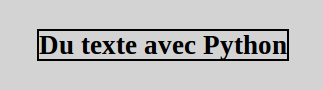
\includegraphics[scale=0.6]{ecran-markdown-2}
\end{center}

\begin{enumerate}
  \item 
  \begin{enumerate}
    \item Définis une fenêtre \ci{tkinter} de taille $800 \times 600$ par exemple.

    \item Dessine un rectangle gris (qui sera notre zone de texte) de taille \ci{largeur} $\times$ \ci{hauteur} (par exemple $700 \times 500$).

    \item Définis plusieurs types de fontes : \ci{fonte_titre}, \ci{fonte_sous_titre}, \ci{fonte_gras}, \ci{font_italique}, \ci{fonte_texte}.
    
    \item Affiche des textes avec différentes fontes.
  \end{enumerate}
    
  \item Écris une fonction \ci{encadre_mot(mot,fonte)} qui dessine un rectangle autour d'un texte. Pour cela utilise la méthode \ci{canvas.bbox(monobjet)} qui renvoie les coordonnées $x_1,y_1,x_2,y_2$ du rectangle voulu. (Ici \ci{monobjet = canvas.create_text(...)}).
  
  \item Écris une fonction \ci{longueur_mot(mot,fonte)} qui calcule la longueur d'un mot en pixels (c'est la largeur du rectangle de la question précédente).
  
  \item Écris une fonction \ci{choix_fonte(mode,en_gras,en_italique)} qui renvoie le nom d'une fonte adaptée (parmi celles définies en première question) selon un mode (parmi \ci{"titre"}, \ci{"sous_titre"}, \ci{"texte"}) et selon des booléens \ci{en_gras}, \ci{en_italique}.
  
  Par exemple \ci{choix_fonte("texte",True,False)} renvoie la fonte \ci{fonte_gras}.
\end{enumerate}

\end{activite}


%%%%%%%%%%%%%%%%%%%%%%%%%%%%%%%%%%%%%%%%%%%%%%%%%%%%%%%%%%%%%%%%
%%%%%%%%%%%%%%%%%%%%%%%%%%%%%%%%%%%%%%%%%%%%%%%%%%%%%%%%%%%%%%%%

\begin{cours}[Markdown]
Le \emph{Markdown}\index{markdown@\emph{markdown}} est un langage de balisage simple qui permet d'écrire un fichier texte  propre et éventuellement de le convertir vers un autre format (html, pdf\ldots).

Voici un exemple de fichier texte avec une syntaxe \emph{Markdown} avec juste en dessous son rendu graphique.
\begin{center}
\footnotesize
\begin{minipage}{0.7\textwidth}
\begin{verbatim}
# L’Origine des Espèces
## par Charles Darwin

Les rapports géologiques qui existent entre la ** faune 
actuelle ** et la ** faune éteinte ** de l’Amérique 
méridionale, ainsi que certains faits relatifs à la 
distribution des êtres organisés qui peuplent ce continent, 
m’ont profondément frappé lors de mon voyage à bord du 
navire le * Beagle * en qualité de naturaliste.

** Chapitres ** 

+ De la variation des espèces à l’état domestique.
+ De la variation à l’état de nature.
+ La lutte pour l’existence.
+ La sélection naturelle ou la persistance du plus apte.
+ ...
\end{verbatim}
\end{minipage}
\end{center}
\begin{center}
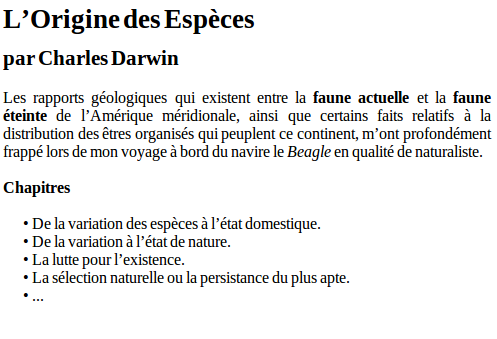
\includegraphics[scale=0.6]{ecran-markdown-1}
\end{center}


La syntaxe est simple, avec un fichier texte bien lisible. Voici quelques éléments de cette syntaxe :
\begin{itemize}
  \item un \textbf{texte en gras} s'obtient en entourant le texte par deux astérisques \ci{**} ;
  \item un \emph{texte en italique} s'obtient en entourant le texte par un astérisque \ci{*} ;
  \item la ligne d'un titre commence par dièse \# ;
  \item la ligne d'un sous-titre commence par deux dièses \#\# ;
  \item pour les éléments d'une liste, chaque ligne commence par un symbole spécial, pour nous ce sera le symbole \og{}plus\fg{} \ci{+}.
  \item Il existe aussi une syntaxe pour afficher des liens, des tableaux, du code\ldots 
\end{itemize}

Dans la suite nous utiliserons la syntaxe simplifiée comme elle est décrite ci-dessus.
\end{cours}

%%%%%%%%%%%%%%%%%%%%%%%%%%%%%%%%%%%%%%%%%%%%%%%%%%%%%%%%%%%%%%%%
% Activité 2
%%%%%%%%%%%%%%%%%%%%%%%%%%%%%%%%%%%%%%%%%%%%%%%%%%%%%%%%%%%%%%%%

\begin{activite}[Visualiser du \emph{Markdown}]

\objectifs{Objectifs : visualiser du texte avec la syntaxe \emph{Markdown} simplifiée.}

\begin{enumerate}
  \item Écris une fonction \ci{afficher_ligne_v1(par,posy)} qui affiche \emph{un par un} les mots d'un paragraphe \ci{par} (sur la ligne d'ordonnée \ci{posy}). 
  
\begin{center}

\includegraphics[scale=0.6]{ecran-markdown-3}
\end{center}   

  Indications :
  \begin{itemize}
    \item Ces mots sont obtenus grâce à la commande \ci{par.split()}.
    \item La ligne affichée commence tout à gauche, elle déborde à droite si elle trop longue.
    \item Après chaque mot on place une espace puis le mot suivant.
    \item Sur l'image ci-dessus les mots sont encadrés.
   \end{itemize}
   
 
  \item Améliore ta fonction en \ci{afficher_ligne_v2(par,posy)} pour tenir compte des titres, sous-titres et listes.
  
   
\begin{center}
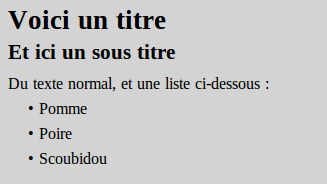
\includegraphics[scale=0.7]{ecran-markdown-4}
\end{center}    
  
  Indications :
  \begin{itemize}
    \item Pour savoir dans quel mode il faut afficher la ligne, il suffit de tester les premiers caractères de la ligne. La ligne d'un titre commence par \#, celle d'un sous-titre par \#\#, celle d'une liste par \ci{+}. 
    
    \item Pour les listes, tu peux obtenir le caractère \og{}\textbullet\fg{} par le caractère unicode \ci{u'\\u2022'}\index{unicode}. Tu peux aussi indenter les éléments de la liste pour plus de lisibilité.
    
    \item Utilise la fonction \ci{choix_fonte()} de la première activité.
    
    \item Sur l'image ci-dessus, chaque ligne est produite par un appel à la fonction. Par exemple \ci{afficher_ligne_v2("## Et ici un sous titre",100)}
   \end{itemize}


  \item Améliore encore ta fonction en \ci{afficher_ligne_v3(par,posy)} pour tenir compte des mots en gras et en italique dans le texte.
  
\begin{center}
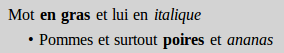
\includegraphics[scale=0.7]{ecran-markdown-5}
\end{center}   
 
   Indications :
  \begin{itemize}
    \item Les mots en gras sont entourés par la balise \ci{**}, les mots en italique par la balise \ci{*}. Dans notre syntaxe simplifiée, les balises sont séparées des mots par des espaces, par exemple : \lstinline!"Mot ** en gras ** et lui en * italique *"!.
    
    
    \item Définis une variable booléenne \ci{en_gras} qui est fausse au départ ; chaque fois que tu rencontres la balise \ci{**} alors inverse la valeur de \ci{en_gras} (\og{}vrai\fg{} devient \og{}faux\fg{}, \og{}faux\fg{} devient \og{}vrai\fg{}). Tu peux utiliser l'opérateur \ci{not}.
    
    \item Utilise encore la fonction \ci{choix_fonte()} de la première activité.
    
    \item Sur l'image ci-dessus, chaque ligne est produite par un appel à la fonction. Par exemple \ci{afficher_ligne_v3("+ Pommes et surtout ** poires ** et * ananas *",100)}
   \end{itemize} 
   
   
  \item Améliore encore ta fonction en \ci{afficher_paragraphe(par,posy)} qui gère l'affichage d'un paragraphe (c'est-à-dire une chaîne de caractères qui peut être très longue) sur plusieurs lignes.
  
\begin{center}
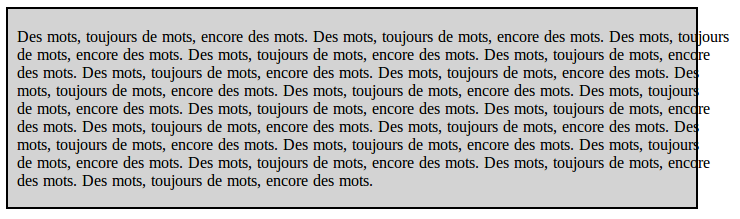
\includegraphics[scale=0.6]{ecran-markdown-6}
\end{center}   
 
   Indications :
  \begin{itemize}
    \item Dès que l'on place un mot qui dépasse la longueur de la ligne (voir ceux qui sortent du cadre sur l'image ci-dessus), alors le mot suivant est placé sur la ligne suivante.
    
    \item La fonction va donc modifier la variable \ci{posy} à chaque saut de ligne. À la fin, la fonction retourne la nouvelle valeur de \ci{posy}, qui sera utile pour afficher le paragraphe suivant.
 
   \end{itemize}    
   
   \item Termine par une fonction \ci{afficher_fichier(nom)} qui visualise les paragraphes d'un fichier texte ayant la syntaxe \emph{Markdown} simplifiée.
\end{enumerate} 
\end{activite}

%%%%%%%%%%%%%%%%%%%%%%%%%%%%%%%%%%%%%%%%%%%%%%%%%%%%%%%%%%%%%%%%
% Activité 3
%%%%%%%%%%%%%%%%%%%%%%%%%%%%%%%%%%%%%%%%%%%%%%%%%%%%%%%%%%%%%%%%

\begin{activite}[Justification]

\objectifs{Objectifs : comprendre comment il est possible de \og{}justifier\fg{} un texte, c'est-à-dire de faire en sorte que les mots soient bien alignés sur la partie gauche et la partie droite de la page. Pour modéliser le problème nous travaillons avec une suite d'entiers qui représente les longueurs de nos mots.}


Dans cette activité :
\begin{itemize}
 \item  \ci{longueurs} est une liste d'entiers (par exemple une liste de $50$ entiers compris entre $5$ et $15$) qui représentent les longueurs des mots ;
 \item on fixe une constante \ci{longueur_ligne} qui représente la longueur d'une ligne. Pour nos exemples, cette longueur vaut $100$.
 \end{itemize}


Dans les activités précédentes, nous passions à la ligne suivante après qu'un mot ait dépassé la fin de ligne.
Nous représentons ceci par la figure suivante :
\begin{center}
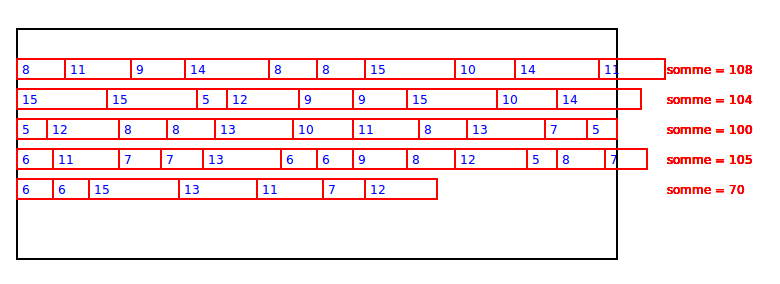
\includegraphics[scale=0.5]{ecran-coupures-1}
\end{center} 
Tu vas essayer de placer les mots plus joliment !

Les dessins sont construits sur la base de l'exemple :
\begin{center}
\ci{longueurs =} [8, 11, 9, 14, 8, 8, 15, 10, 14, 11, 15, 15, 5, 12, 9, 9, 15, 10, 14, 5, 12, 8, 8, 13, 10, 11, 8, 13, 7, 5, 6, 11, 7, 7, 13, 6, 6, 9, 8, 12, 5, 8, 7, 6, 6, 15, 13, 11, 7, 12]
\end{center}

qui a été obtenu par un tirage aléatoire grâce aux commandes :\\
\begin{lstlisting}
from random import randint
longueurs = [randint(5,15) for i in range(50)]
\end{lstlisting}


\begin{enumerate}
  \item Écris une fonction \ci{coupures_simples()} qui calcule les indices permettant de réaliser les coupures correspondant à la figure ci-dessous, c'est-à-dire un alignement à gauche (sans espaces) et sans dépasser la longueur totale de la ligne (ici de longueur $100$).
  
\begin{center}
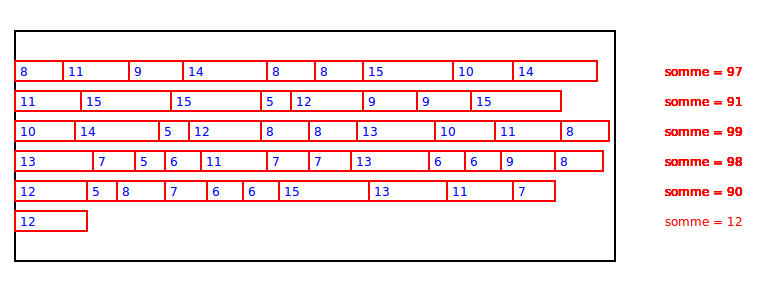
\includegraphics[scale=0.5]{ecran-coupures-2}
\end{center} 

  \begin{fonction}[\ci{coupures_simples()}]
  Usage : \ci{coupures_simples(long)} \\
  Entrée : une suite de longueurs (une liste d'entiers)\\
  Sortie : la liste des indices où effectuer une coupure
  \medskip
    
  Exemple : \ci{coupures_simples(longueurs)} où \ci{longueurs} est l'exemple donné ci-dessus, renvoie la liste \ci{[0, 9, 17, 27, 39, 49, 50]}. C'est-à-dire que :
  \begin{itemize}
    \item la première ligne correspond aux indices $0$ à $8$ (donnés par \ci{range(0,9)}),
    \item la deuxième ligne  correspond aux indices $9$ à $16$ (donnés par \ci{range(9,17)}),
    \item la troisième ligne correspond aux indices $17$ à $26$ (donnés par \ci{range(17,27)}),
    \item \ldots
    \item la dernière ligne correspond à l'indice $49$ (donné par \ci{range(49,50)}).
    \end{itemize}
             
  \end{fonction}

  \item Modifie ton travail en une fonction \ci{coupures_espaces()} qui rajoute une espace (avec \ci{longueur_espace = 1}) entre deux mots d'une même ligne (mais pas au début de ligne, ni à la fin de la ligne). Cela correspond au dessin suivant :
  
\begin{center}
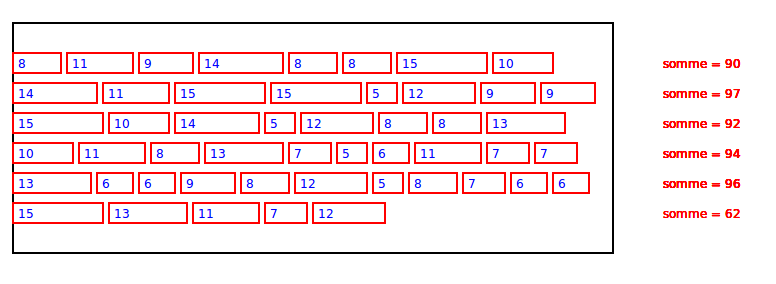
\includegraphics[scale=0.5]{ecran-coupures-3}
\end{center} 

Pour notre exemple, les coupures renvoyées sont \ci{[0, 8, 16, 24, 34, 45, 50]}.


  \item Afin de pouvoir justifier le texte, tu autorises les espaces à être plus grandes que la longueur initiale de $1$. Sur chaque ligne, les espaces entre les mots sont toutes de la même longueur (supérieure ou égale $1$) de sorte que le dernier mot soit aligné à droite. D'une ligne à l'autre, la longueur des espaces peut changer.
 
\begin{center}
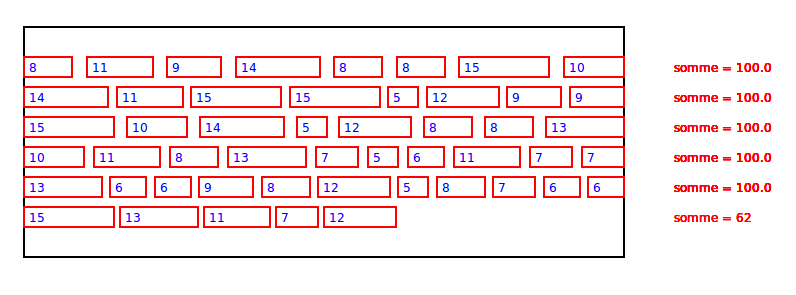
\includegraphics[scale=0.5]{ecran-coupures-4}
\end{center}

Écris une fonction \ci{calcul_longueur_espaces()} qui renvoie la longueur que doivent avoir les espaces de chaque ligne pour que le texte soit justifié.
Pour notre exemple, on obtient la liste \ci{[2.43, 1.43, 2.14, 1.67, 1.40, 1.00]}, c'est-à-dire que pour la première ligne les espaces doivent être de longueur $2.43$, pour la seconde  $1.43$,\ldots 

Pour trouver la formule qui convient, il suffit de reprendre les résultats de la fonction \ci{coupures_espaces()} puis, pour chaque ligne, compter le nombre de mots qu'elle contient, ainsi que la valeur qu'il manque pour arriver au total de $100$.
\end{enumerate} 
\end{activite}


\bigskip
\bigskip

\objectifs{Tu as maintenant tout en main pour visualiser du texte écrit avec la syntaxe \emph{Markdown} et le justifier. Cela représente quand même encore du travail ! Tu peux aussi améliorer la prise en charge de la syntaxe \emph{Markdown} : prendre en charge le code, les listes numérotées, les sous-listes, les mots en gras et en italique en même temps\ldots}


\end{document}
